\section{Prototype Description}\label{sec:PrototypeDescription}
In the following section an overall description of the prototype is given. %This is done to help the reader understand the utilized setup in the project.
The prototype is divided into three separate subsystems. The quadcopter, the ground station, and the Vicon system. These can be seen in \autoref{fig:prototypediagram}. 
\vspace{-0.2 cm}
\begin{figure}[H]
  \centering
  \captionbox
  {
    Schematic diagram of the prototype, which includes the quadcopter, the ground station and the Vicon system.
    \label{fig:prototypediagram}
  }
  {
    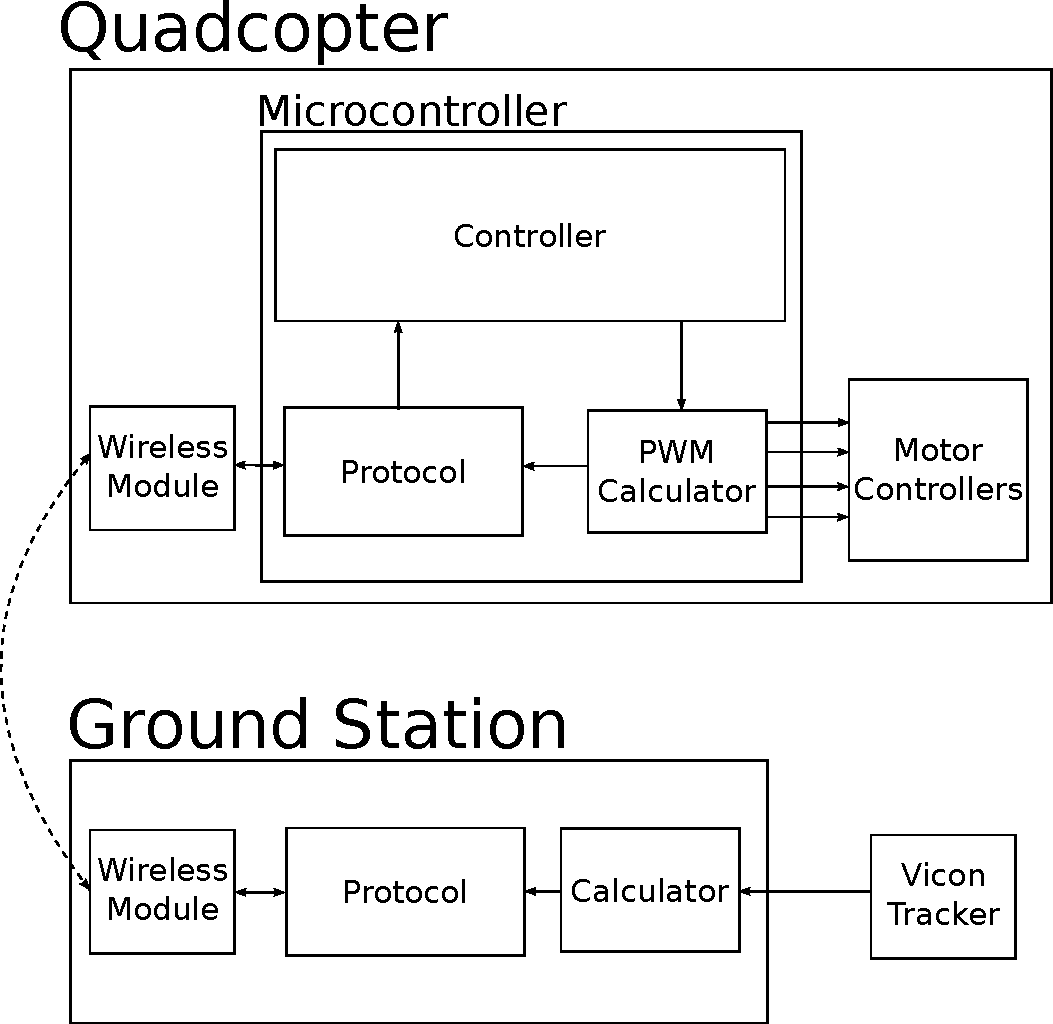
\includegraphics[width=.45\textwidth]{figures/prototypediagram}
  }
\end{figure}
\vspace{-0.7 cm}
%For this project the Vicon system is used to capture the position and orientation of the quadcopter. It captures the quadcopter's position, in form of coordinates, and its orientation, in the form of Euler angles. The information is then transmitted to the Ground Station.
%The Ground Station utilizes the data it receives from the Vicon system to calculate the linear velocity and linear acceleration of the quadcopter.
The Vicon system captures the quadcopter's position, in form of coordinates, and its attitude, in Euler angles. This information is then transmitted to the Ground Station. It is desired to move the quadcopter in the x, y and z directions. The reference commands are therefore transmitted together with the position, attitude and calculated translational velocities to the controller placed on the quadcopter.

The information is transmitted by means of a network interface through the XBees. The function protocol is implemented in the Ground Station to be able to generate a packet which can be transmitted and decoded on the micro controller. It is also needed for the micro controller to detect packets and disregard incorrect packets.

The quadcopter consists of a microcontroller, four motor controllers, four motors, a battery, and a wireless module. The microcontroller's tasks are to handle the network between itself and the ground station, the control calculations and to generate the control signals which should be applied to the four motor controllers.

To be able to calculate the rotational speed needed for the motors, the variables received from the ground station are needed, i.e the control reference, position, attitude and translational velocities of the quadcopter. Hereafter it is possible to calculate the necessary PWM signals, by utilizing the rotational speed calculated by the control system and the relationship between the rotational speed and the PWM signal, found in \autoref{app:duty}.
% and the measured voltage on the battery. 
%Furthermore, the quadcopter should be able to measure the battery voltage level and land when the battery is critically low.
%to the ground station in order to detect when the flight should end.
%The quadcopter's most complex component is the microcontroller. It handles the control calculations, the PWM calculations according to the required control action and battery level, and the communication protocol necessary to exchange data with the ground station.
%The microcontroller requires 4 PWM outputs with different and independent duty cycles for controlling the 4 motors in the quadcopter. 
%The network interface in the microcontroller handles the incoming data from the ground station. This data consist of reference commands for the controllers and sensor data. It should also be able to send the battery voltage level to the ground station in order to detect when to end the flight.
%The communication between the ground station and the quadcopter is done through wireless modules. These should allow the implementation of the communication by designing only the transport layer protocol.
%The ground station gathers the information coming from the Vicon system and sends it to the quadcopter. This also includes doing calculations with the received Vicon data to obtain other variables like velocities or accelerations.
%Finally, Vicon system uses the position of the markers placed in the quadcopter to provide its position and orientation. The orientation data is given in multiple forms but only Euler angles data is considered.
%\textbf{Battery should be moved somewhere else}
%The battery, which is available for the prototype, is a Zippy Flightmax battery. Its weights 141 gram, has an capacity of 1500 mAh, a voltage of 11.1 volts and a discharge current of 20 amperes. 
\vspace{-1.5 cm}